\section{FRONTEND}\label{ch:frontend}

Das Frontend wurde mithilfe des Admin-Dashboard ngx-admin auf Basis von Angular 9+ und Nebular entwickelt. Mittels Angular wird eine Weboberfläche komponentenbasiert zur Verfügung gestellt. Für die serverseitige Anwendung benötigt Angular zudem Node.js, eine JavaScript-Laufzeitumgebung. Zudem wird ngx-admin mit dem Eva Design System unterstützt, um UI-Design zu vereinfachen. 

\subsection{Architektur}

In der UNTEREN ABBILDUNG ist die Architektur des Frontend zu sehen. Eine Komponente besteht aus einem Template (HTML-Datei) und einem Style (SCSS-Datei). Diese werden als Metadaten im Dekorator der Komponente festgelegt und stellen die Ansicht dar. Mithilfe der Datenbindung kann das Template mit der Komponente Daten austauschen und gegebenenfalls Events ausführen. Bei Bedarf können Komponenten durch die Dependency Injection Zugriff auf eine Serviceklasse erhalten. Somit können wiederverwendbare Funktionen oder Daten aus dem Backend zur Verfügung gestellt werden. In den Modulen werden Komponenten, Module, Services usw. gruppiert und verwaltet. In Angular werden zwei Modularten unterschieden. Jedes Angular Projekt besitzt ein Root-Modul, das app.module.ts heißt. Diese ist dazu da, um die gesamte Webanwendung zu verwalten und diese wird beim Start der Anwendung als erstes geladen und initialisiert. Mit Feature-Modulen kann der Code, der sich auf eine bestimmte Funktionalität oder ein bestimmtes Feature bezieht, von anderem Code getrennt werden und bleibt somit organisiert.

\begin{figure}[thpb]
      \centering
      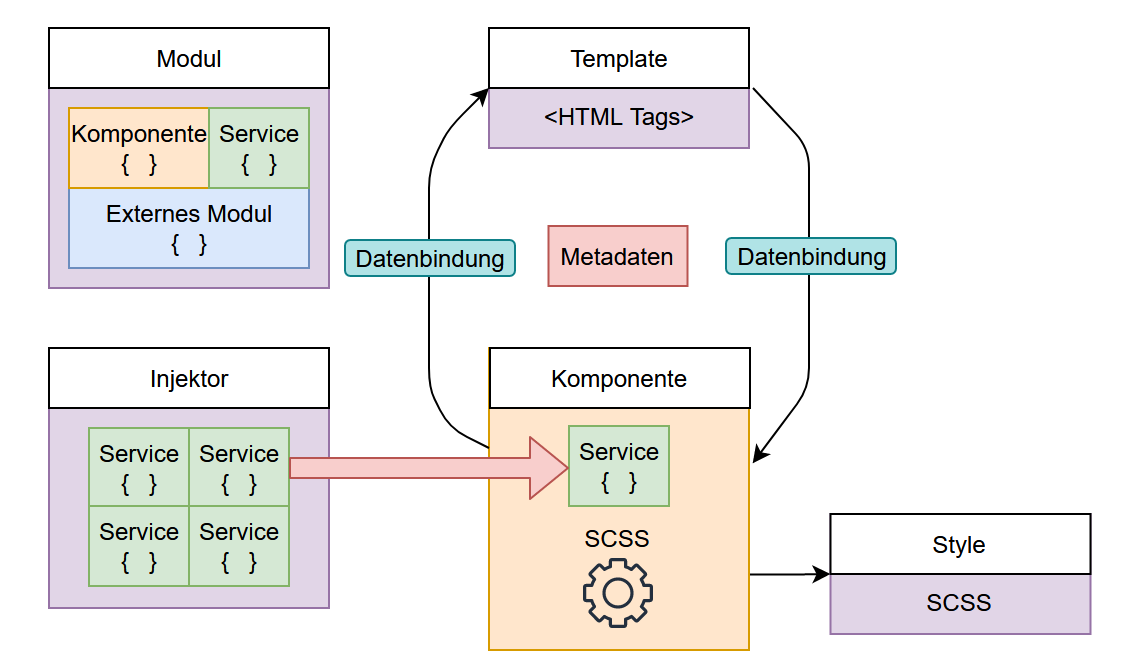
\includegraphics[scale=0.55]{img/frontend_architecture.png}
      \caption{Angular Architektur des Projektes}
      \label{fig:frontend}
 \end{figure}


\subsection{Entwickelte Komponenten}

\item \textbf{AirQuality}:
\item \textbf{Gantt}:
Das Gantt-Diagramm zeigt an, ob jemand im Raum anwesend war oder nicht. Die Anwesenheit wird mit rot als abwesend und grün als anwesend dargestellt.
\item \textbf{lcd-input}:
\item \textbf{lineChartComponent}:
\item \textbf{switch}:
Ein Knopf, der an- und ausgeschaltet werden kann.
\item \textbf{temperatureGauge}:
Zeigt die Temperatur, Luftfeuchtigkeit und Luftdruck in einem Tachometer an.
\item \textbf{tempSensorCard}:
\item \textbf{sensornode-dashbord}:
In dieser Komponente werden die oben genannten Komponenten des jeweiligen Sensorknotens dargestellt.

!!!TODO Services? und ggf Tests?
